\documentclass[a4paper, 12pt]{article}

%%% Работа с русским языком
\usepackage{cmap}					% поиск в PDF
\usepackage{mathtext} 				% русские буквы в формулах
\usepackage[T2A]{fontenc}			% кодировка
\usepackage[utf8]{inputenc}			% кодировка исходного текста
\usepackage[russian]{babel}	% локализация и переносы

%%% Дополнительная работа с математикой
\usepackage{amsmath,amsfonts,amssymb,amsthm,mathtools} % AMS
\usepackage{icomma} % "Умная" запятая: $0,2$ --- число, $0, 2$ --- перечисление

%% Номера формул
%\mathtoolsset{showonlyrefs=true} % Показывать номера только у тех формул, на которые есть \eqref{} в тексте.

%% Шрифты
\usepackage{euscript}	 % Шрифт Евклид
\usepackage{mathrsfs} % Красивый матшрифт

%% Поля
\usepackage[left=2cm,right=2cm,top=2cm,bottom=2cm,bindingoffset=0cm]{geometry}

%% Русские списки
\usepackage{enumitem}
\makeatletter
\AddEnumerateCounter{\asbuk}{\russian@alph}{щ}
\makeatother

%%% Работа с картинками
\usepackage{graphicx}  % Для вставки рисунков
\graphicspath{{images/}{images2/}}  % папки с картинками
\setlength\fboxsep{3pt} % Отступ рамки \fbox{} от рисунка
\setlength\fboxrule{1pt} % Толщина линий рамки \fbox{}
\usepackage{wrapfig} % Обтекание рисунков и таблиц текстом

%%% Работа с таблицами
\usepackage{array,tabularx,tabulary,booktabs} % Дополнительная работа с таблицами
\usepackage{longtable}  % Длинные таблицы
\usepackage{multirow} % Слияние строк в таблице

%% Красная строка
\setlength{\parindent}{2em}

%% Интервалы
\linespread{1}
\usepackage{multirow}

%% TikZ
\usepackage{tikz}
\usetikzlibrary{graphs,graphs.standard}

%% Верхний колонтитул
\usepackage{fancyhdr}
\pagestyle{fancy}

%% Перенос знаков в формулах (по Львовскому)
\newcommand*{\hm}[1]{#1\nobreak\discretionary{}
	{\hbox{$\mathsurround=0pt #1$}}{}}

%% Мои дополнения
\usepackage{float} %Добавляет возможность работы с командой [H] которая улучшает расположение на странице
\usepackage{gensymb} %Красивые градусы
\usepackage{graphicx}               % Импорт изображений
\usepackage{caption} % Пакет для подписей к рисункам, в частности, для работы caption*

% подключаем hyperref (для ссылок внутри  pdf)
\usepackage[unicode, pdftex]{hyperref}

%%% Теоремы
\theoremstyle{plain}                    % Это стиль по умолчанию, его можно не переопределять.
\renewcommand\qedsymbol{$\blacksquare$} % переопределение символа завершения доказательства

\newtheorem{theorem}{Теорема}[section] % Теорема (счетчик по секиям)
\newtheorem{proposition}{Утверждение}[section] % Утверждение (счетчик по секиям)
\newtheorem{definition}{Определение}[section] % Определение (счетчик по секиям)
\newtheorem{corollary}{Следствие}[theorem] % Следстиве (счетчик по теоремам)
\newtheorem{problem}{Задача}[section] % Задача (счетчик по секиям)
\newtheorem*{remark}{Примечание} % Примечание (можно переопределить, как Замечание)
\newtheorem{lemma}{Лемма}[section] % Лемма (счетчик по секиям)

\begin{document}
    \newcommand{\HRule}{\rule{\linewidth}{0.7mm}} % Defines a new command for the horizontal lines, change thickness here
	
	\begin{center}
		\large\textbf{Московский Физико-Технический Институт}\\ % Name of your university/college
		\large\textbf{(государственный университет)}
	
		\vfill
		
		\Large Лабораторная работа по курсу общей физики № *labnum*\\[0.5cm] % Preambule of your document title
		
		
		\HRule
		\\[0.4cm]
		{ \huge \bfseries *name of your labwork*}% Title of your document
		\\[0.4cm] 
		\HRule
		\\[0.5cm]
		
		\ \\
	\textbf{\large Автор:} \\	
	\large *your name* *groupname*\\ % Your name and something more, your group num for example
		\vfill
		\hspace*{-0.8 cm}
\includegraphics[width=100 pt]{frkt_logo}\\ % logo of your  company/university/college
		\large Долгопрудный, 2021 % location and year
	\end{center}

\newpage
\setcounter{page}{2}
\fancyfoot[c]{\thepage}
\fancyhead[L] {Работа № *labnum*} % some information in page header
\fancyhead[R]{}

	\textbf{Цель данной работы:} исследовать проникновение переменного магнитного поля в медный полый цилиндр, оценить глубину проникновения магнитного поля (скиновую глубину) в цилиндр. Рассчитать удельную проводимость меди $\sigma$, сравнив ее с табличной. Получить зависимость коэффициента ослабления магнитного поля $H$ от частоты генератора $f$ и сравнить экспериментальные данные с теорией. 

	\vspace{10mm}
	\textbf{Оборудование, задействованное в работе:} генератор звуковой частоты, соленоид, намотанный на полый цилиндрический каркас из диэлектрика, медный экран в виде трубки, измерительная катушка, амперметр, вольтметр, осциллограф.

	\vspace{20mm}

	\section*{Общая теория скин-эффекта}
	
	\begin{wrapfigure}{l}{0.2\textwidth}
		\vspace{-20pt}
		\begin{center}
			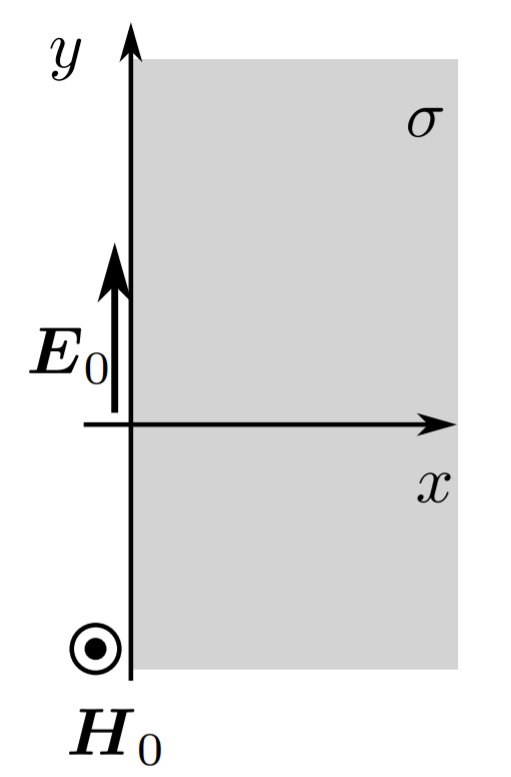
\includegraphics[height=0.2\textheight]{images/Skin1.png}
		\end{center}
		\vspace{-20pt}
		\caption{Скин-эффект в плоской геометрии}
		\vspace{20pt}
	\end{wrapfigure}

	Рассмотрим квазистационарное поле внутри проводящей среды в простейшем плоском случае. Пусть вектор $\boldsymbol{H}$ направлен всюду вдоль оси $z$ и зависит только от координаты $x$, то есть $H_x = H_y \equiv 0$.
	
	
	\noindent Из уравнений Максвелла следует равенство:
	
	\begin{equation}
		\nabla^2\boldsymbol{H} = \sigma\mu\mu_0\dfrac{\partial\boldsymbol{H}}{\partial t}.
	\end{equation}
	
	\noindent В нашем случае оно примет вид:
	
	\begin{equation}
		\dfrac{\partial^2 H_z}{\partial x^2} = \sigma\mu\mu_0 \dfrac{\partial H_z}{\partial t}.
	\end{equation} 

	\noindent Пусть полупространство $x > 0$ заполнено проводящей средой с проводимостью $\sigma$, а на границе $x = 0$ задано магнитное поле, изменяющееся по гармоническому закону: $H_z = H_0 e^{i\omega t}$. Будем искать решение уравнения выше также в виде гармонической функции: $H_z(x, t) = H(x)e^{i\omega t}$.
	
	\noindent После подстановки в уравнение получим:
	
	\begin{equation}
		\dfrac{d^2 H}{dx^2} = i\omega\sigma\mu\mu_0H.
		\label{H_diff}
	\end{equation}

	\noindent Как известно из теории линейных дифференциальных уравнений,
	решение нужно искать в виде: $H(x) = H_0 e^{k x}$. Подставляя, получим,
	что уравнение имеет нетривиальные решения такого вида при $k^2 = i\omega\sigma\mu\mu_0$. Откуда получаем:
	
	\begin{equation}
		k = \pm \dfrac{1+i}{\sqrt{2}}\sqrt{\omega\sigma\mu\mu_0}.
	\end{equation}

	\noindent Для полубесконечной среды $(z > 0)$ физический смысл имеет только решение со знаком минус, соответствующее стремлению к нулю амплитуды поля при $z \rightarrow \infty$. Окончательное решение уравнения:
	
	\begin{equation}
		H_z(x, t) = H_0e^{-x/\delta}e^{i(\omega t - x/\delta)},
	\end{equation}

	\noindent где $\delta = \sqrt{\dfrac{2}{\omega\sigma\mu\mu_0}} = \dfrac{1}{\sqrt{\pi f \sigma\mu\mu_0}}$ - \textbf{глубина проникновения} поля, или \textbf{скиновая} глубина.
	
	\newpage

	\section*{Специфика работы}
	
	\begin{figure}[h!]
		\centering
		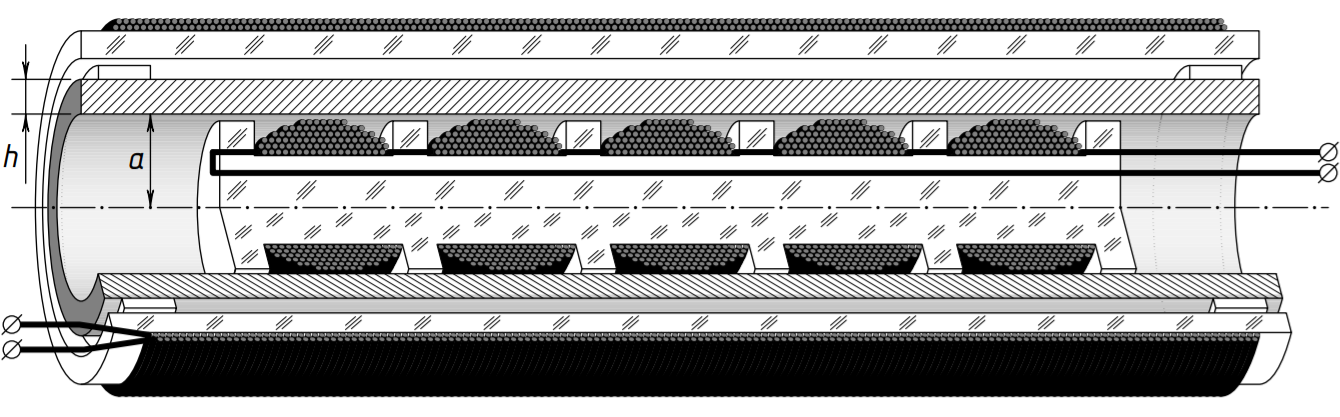
\includegraphics[scale=0.6]{images/Skin2.png}
		\caption{Тонкостенный цилиндр}
	\end{figure}
	
	В работе изучается скин-эффект в длинном тонкостенном медном цилиндре, помещённом внутрь соленоида, поэтому $\mu \approx 1$ с хорошей точностью.
	
	Если выполнено условие $h \ll a$, то для описания поля внутри стенки можно ограничиться одномерным приближением. После решения уравнения (\ref{H_diff}) и подстановки граничных условий $H(0) = H_0$, $H(h) = H_1$ приходим к главной формуле всей работы:
	
	\begin{equation}
		H_{1} = \dfrac{H_0}{\frac{1}{2}ak \sh{k h} + \ch{k h}}
	\end{equation}

	Разобьем на предельные случаи.
	
	\begin{enumerate}
		\item \textbf{Малые частоты.}
			Имеем $\delta \gg h$, откуда $|kh| \ll 1$, значит $\ch kh \approx 1, \sh kh \approx kh$, и тогда:
			
			\begin{equation}
				H_1 \approx \dfrac{H_0}{1 + i\frac{ah}{\delta^2}}.
			\end{equation}
		
			Следовательно для отношения модулей получаем:
			\begin{equation}
				\dfrac{|H_1|}{|H_0|} = \dfrac{1}{\sqrt{1+ \left(\frac{ah}{\delta^2}\right)^2}} = \dfrac{1}{\sqrt{1 + \frac{1}{4}\left(ah\sigma\mu_0\omega\right)^2}} = \dfrac{1}{\sqrt{1 + \left(ah\pi f\sigma\mu_0\right)^2}}.
			\end{equation}
		
		 	А фаза $H_1$ отстает от фазы $H_0$ на $\psi = \arctg\left(\dfrac{ah}{\delta^2}\right)$.
		 	
		 \item \textbf{Большие частоты.} 
		 	Ситуация обратная -- $\delta \ll h$. Тогда $|kh| \gg 1$ и 	$|ka| \gg 1$, откуда $\sh kh \approx \ch kh \approx \dfrac{1}{2}e^{kh}$, и тогда:
		 
		 	\Large
			\begin{equation}
			 	\frac{H_1}{H_0} = \frac{4}{ka}e^{-kh} = \frac{2\sqrt{2}\delta}{a}e^{-\frac{h}{\delta}}e^{-i\left(\frac{\pi}{4} + \frac{h}{\delta}\right)}.
			 	\label{high}
			\end{equation}
	\end{enumerate}
	
	\newpage
	
	Как видно из формулы (\ref{high}), в этом пределе поле внутри цилиндра по модулю в $\frac{2\sqrt{2}\delta}{a}e^{-h/\delta}$ раз меньше, чем снаружи, и, кроме того, запаздывает по фазе на:
	
	\begin{equation}
		\psi = \frac{\pi}{4} + \frac{h}{\delta} = \frac{\pi}{4} + h\sqrt{\pi f \sigma\mu_0}.
		\label{freq}
	\end{equation}
	
	\vspace{60mm}
	\section*{Экспериментальная установка}
	\begin{figure}[h!]
		\centering
		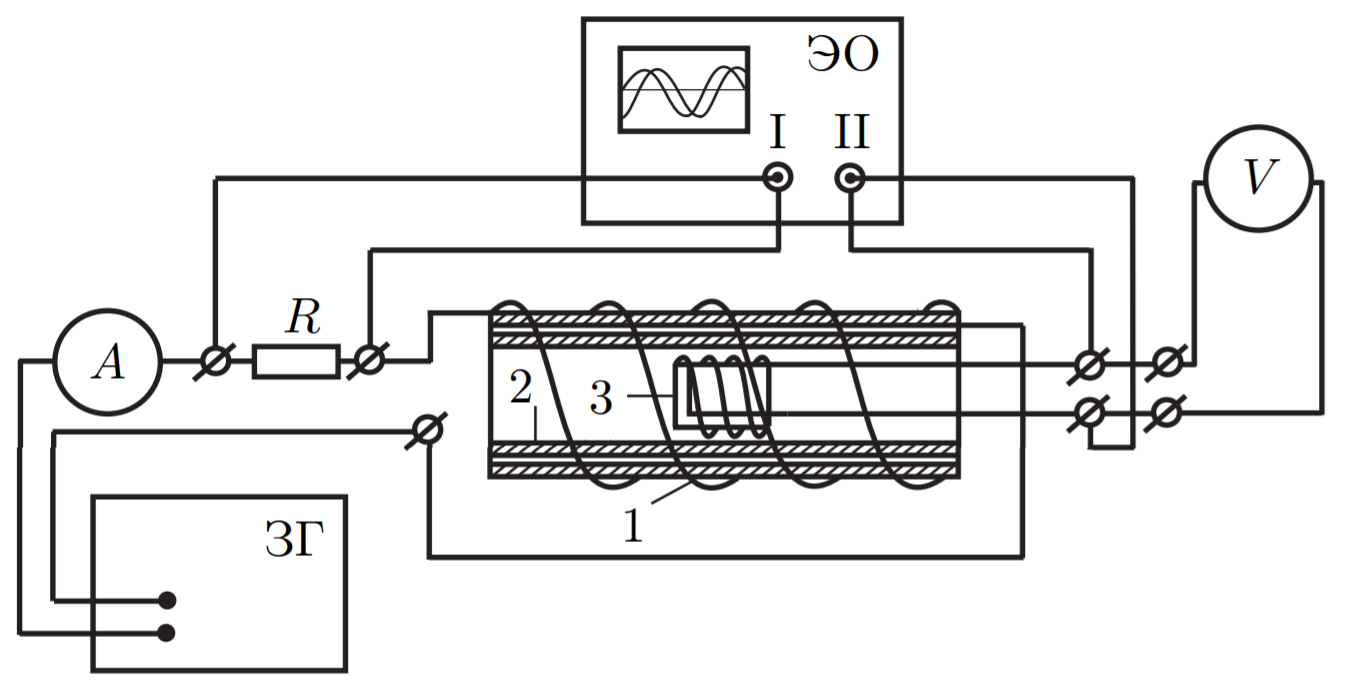
\includegraphics[scale=0.5]{images/Scheme.png}
		\caption{Экспериментальная установка для изучения скин-эффекта}
	\end{figure}

	Схема экспериментальной установки для исследования проникновения переменного магнитного поля в медный полый цилиндр изображена на рис. 3. Переменное магнитное поле создаётся с помощью соленоида, намотанного на полый цилиндрический каркас 1 из поливинилхлорида, который подключается к генератору звуковой частоты. Внутри соленоида расположен медный цилиндрический экран 2. Для измерения магнитного поля внутри экрана используется измерительная катушка 3.
	
	С помощью вольтметра $V$ измеряется действующее значение ЭДС индукции, которая возникает в измерительной катушке, находящейся в переменном магнитном поле $H_1 e^{i\omega t}$. Комплексная амплитуда ЭДС индукции в измерительной катушке равна 
	\begin{equation*}
		\widehat{U} = -SN \frac{d\widehat{B_1}(t)}{dt} = -i\omega\mu_0 SN H_1 e^{i\omega t}.
	\end{equation*}
	
	Показания вольтметра, измеряющего это напряжение, будут тогда, соответственно, равны:
	\begin{equation*}
		U = \frac{SN\omega}{\sqrt{2}}\mu_0 |H_1|.
	\end{equation*}

	Видно, что модуль амплитуды магнитного поля внутри экрана $|H_1|$ пропорционален $U$ и обратно пропорционален частоте сигнала $f$:
	\begin{equation*}
		|H_1| \propto \frac{U}{f}.
	\end{equation*}

	При этом поле вне экрана $|H_0|$ пропорционально току $I$ в цепи соленоида, измеряемому амперметром $A$:
	\begin{equation*}
		|H_0| \propto I.
	\end{equation*} 

	Следовательно:
	\begin{equation}
		\frac{|H_1|}{|H_0|} = \text{const} \cdot \frac{U}{fI}
	\end{equation}

	Таким образом, отношение амплитуд магнитных полей снаружи и
	вне экрана (коэффициент ослабления) может быть измерено по отношению $\frac{U}{fI}$ при разных частотах, а неизвестная константа в соотношении может быть определена по измерениям при малых частотах.
	
	\vspace{90mm}
	\section*{Определение проводимости материала экрана}
	В установке в качестве экрана используется медная труба промышленного производства. Технология изготовления труб оказывает заметное влияние на электропроводимость. Из-за наличия примесей проводимость меди трубы в данной работе отличается от табличного значения в меньшую сторону. Для определения $\sigma$ экрана будем использовать частотную зависимость (\ref{freq}) фазового сдвига между магнитными полями внутри и вне экрана при высоких частотах. Как видно из выражения (\ref{freq}), в области больших частот $f \gg \frac{1}{h^2 \pi \sigma\mu_0}$ зависимость $\psi(\sqrt{f})$ аппроксимируется прямой, проходящей через точку $\psi(0) = \frac{\pi}{4}$. По наклону этой прямой можно вычислить проводимость материала экрана.
	
	
	
	\newpage
    \section*{Ход работы}

    %% подписать что есть что
    \begin{center}
        Запишем параметры установки \\
        $a = (22.5 ~ \pm ~ 0.5)$ мм -- радиус цилиндра \\
        $h = (1.5 ~ \pm ~ 0.1)$ мм -- толщина стенок
    \end{center}

    \begin{enumerate}
        \item Сняли зависимость $U(f)$ и $I(f)$ в области низких частот: 10-100 Гц для получения зависимости
        амплитуды магнитного поля внутри экрана от частоты $\xi_{0c}(f)$. Результаты измерений приведены в таблице %какой.

        \begin{equation}
            \xi_{0c} = \frac{U}{f I}
        \end{equation}

        \item Одновременно исследовали зависимость $\xi_{0c}$ и фазового сдвига $\Delta \psi$ от частоты в диапазоне высоких частот
        0.1-35 кГц. Результаты измерений приведены в таблице %какой.
        \\

        \textbf{Замечание:} сдвиг фазы $\Delta \varphi$, измеренный по экрану осциллографа, будет отличаться от
        фазового сдвига между магнитными полями вне и внутри экрана на $\pi/2$.

        \[ \Delta \psi = \Delta \varphi + \frac{\pi}{2} \]
    \end{enumerate}

    \begin{table}[h!]
    \centering
    \begin{tabular}{|c|c|c|c|}
    \hline
    $f$, Гц & $I$, мА & $U$, мВ  & $\xi_{0c} \cdot 10^{-3}$ \\ \hline
    10      & 449,80  & 86,3     & 19,19                    \\ \hline
    20      & 452,47  & 172,0    & 19,01                    \\ \hline
    30      & 449,65  & 254,2    & 18,84                    \\ \hline
    40      & 445,28  & 331,7    & 18,62                    \\ \hline
    50      & 439,86  & 403,5    & 18,35                    \\ \hline
    60      & 433,75  & 469,3    & 18,03                    \\ \hline
    70      & 427,23  & 528,8    & 17,68                    \\ \hline
    80      & 420,61  & 582,0    & 17,30                    \\ \hline
    90      & 413,93  & 629,4    & 16,89                    \\ \hline
    100     & 407,56  & 671,3    & 16,47                    \\ \hline
    \end{tabular}
    \caption{Данные в диапазоне низких частот}
    \label{table_low_f}
\end{table}

    \begin{table}[]
    \centering
    \begin{tabular}{|c|c|c|c|c|c|}
    \hline
    $f$, Гц & $I$, мА  & $U$, мВ   & $\xi_{0c} \cdot 10^{-6}$  & $\Delta \varphi$ & $\Delta \psi$ \\ \hline
    100     & 407,56   & 671,3     & 16 471,19                 & -1,00            & 0,57          \\ \hline
    500     & 316,84   & 966,0     & 6 097,71                  & -0,23            & 1,34          \\ \hline
    1000    & 279,48   & 884,0     & 3 163,02                  & 0,00             & 1,57          \\ \hline
    2000    & 209,62   & 662,2     & 1 579,52                  & 0,20             & 1,77          \\ \hline
    3000    & 159,35   & 496,8     & 1 039,22                  & 0,35             & 1,92          \\ \hline
    4000    & 126,14   & 385,7     & 764,43                    & 0,49             & 2,06          \\ \hline
    5000    & 103,39   & 310,4     & 600,44                    & 0,64             & 2,21          \\ \hline
    6000    & 87,14    & 253,5     & 484,85                    & 0,81             & 2,38          \\ \hline
    7000    & 74,99    & 211,7     & 403,29                    & 0,90             & 2,47          \\ \hline
    8000    & 65,48    & 180,4     & 344,38                    & 0,94             & 2,51          \\ \hline
    9000    & 57,86    & 153,8     & 295,35                    & 1,09             & 2,66          \\ \hline
    10000   & 51,56    & 133,8     & 259,50                    & 1,22             & 2,79          \\ \hline
    12000   & 41,22    & 10,1      & 20,46                     & 1,57             & 3,14          \\ \hline
    14000   & 33,90    & 80,0      & 168,55                    & 1,79             & 3,36          \\ \hline
    15000   & 30,82    & 71,7      & 155,09                    & 1,89             & 3,46          \\ \hline
    16000   & 28,03    & 64,6      & 144,07                    & 1,90             & 3,47          \\ \hline
    17000   & 25,48    & 58,8      & 135,73                    & 1,92             & 3,49          \\ \hline
    18000   & 23,14    & 53,5      & 128,45                    & 2,04             & 3,61          \\ \hline
    19000   & 20,96    & 49,1      & 123,27                    & 2,15             & 3,72          \\ \hline
    20000   & 18,93    & 45,2      & 119,36                    & 2,18             & 3,75          \\ \hline
    21000   & 17,03    & 42,0      & 117,45                    & 2,24             & 3,81          \\ \hline
    22000   & 15,23    & 39,1      & 116,70                    & 2,34             & 3,91          \\ \hline
    23000   & 13,52    & 36,6      & 117,67                    & 2,47             & 4,04          \\ \hline
    24000   & 11,90    & 34,3      & 120,12                    & 2,52             & 4,09          \\ \hline
    25000   & 10,34    & 32,4      & 125,29                    & 2,60             & 4,17          \\ \hline
    26000   & 8,85     & 30,6      & 132,93                    & 2,65             & 4,22          \\ \hline
    27000   & 7,42     & 29,0      & 144,70                    & 2,72             & 4,29          \\ \hline
    28000   & 6,10     & 27,4      & 160,42                    & 2,77             & 4,34          \\ \hline
    29000   & 4,83     & 26,0      & 185,51                    & 2,87             & 4,44          \\ \hline
    30000   & 3,60     & 24,0      & 222,22                    & 2,99             & 4,56          \\ \hline
    31000   & 2,76     & 22,0      & 257,22                    & 3,14             & 4,71          \\ \hline
    32000   & 2,38     & 20,8      & 273,11                    & 3,33             & 4,90          \\ \hline
    33000   & 2,70     & 18,9      & 212,51                    & 3,67             & 5,24          \\ \hline
    34000   & 3,51     & 17,0      & 142,26                    & 4,04             & 5,61          \\ \hline
    35000   & 4,57     & 15,0      & 93,78                     & 4,71             & 6,28          \\ \hline
    \end{tabular}
    \caption{Данные в диапазоне высоких частот}
    \label{table_hight_f}
\end{table}

    \section*{Обработка результатов}

    В области низких частот построим график $\xi_{0c}(f^2)$.

    \begin{figure}[h!]
        \centering
        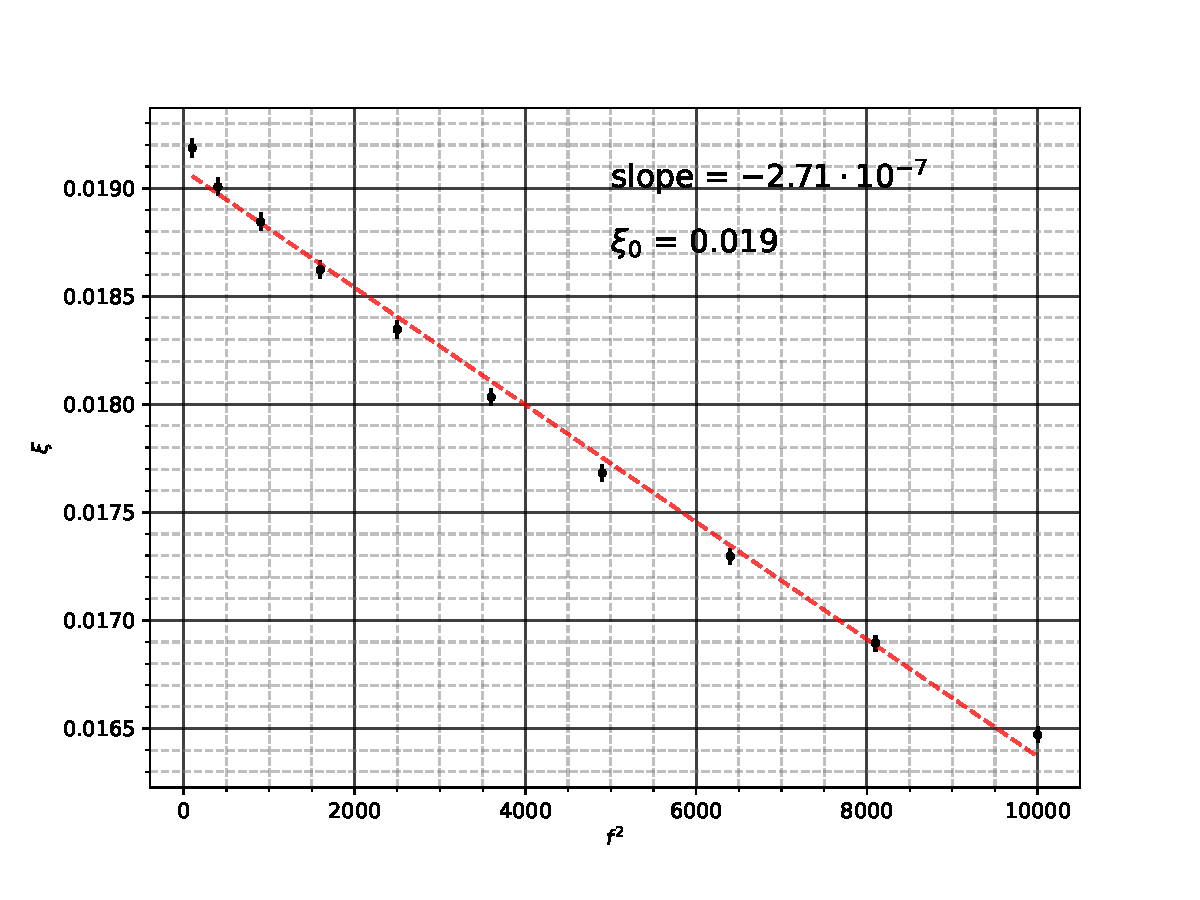
\includegraphics[width = \textwidth]{xi0c(1).pdf}
        \caption{График зависимости $\xi_{0c}$ от $f^2$}
        \label{xi0c(1)}
    \end{figure}

    Экстраполируя прямую к $f = 0$ найдем амплитуду внешнего поля $\xi_0$:

    \begin{center}
        \fbox{$\xi_0 = (1.9000 ~ \pm ~ 0.0037) \cdot 10^{-2}$}
    \end{center}

    Изобразим зависимость частоты фазового сдвига $\Delta \psi$ от $\sqrt{f}$ в диапазоне высоких частот.
    Проведем наилучшую прямую, заметим, что при $f = 0$ значение ординаты $y_0 = 0.75 \approx \pi/4$.

    \begin{figure}
        \centering
        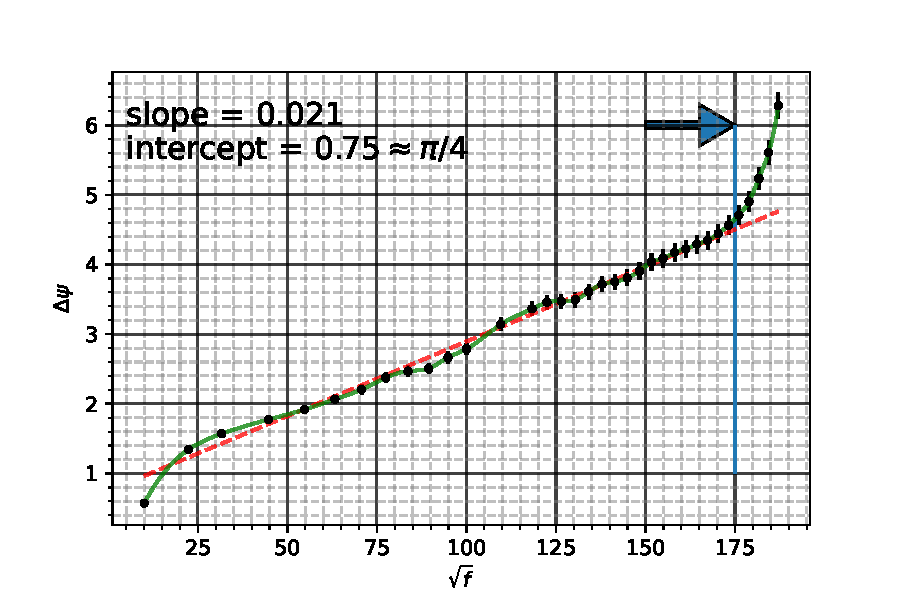
\includegraphics[width = \textwidth]{DeltaPsi.pdf}
        \caption{График зависимости $\Delta \psi$ от $\sqrt{f}$}
        \label{DeltaPsi}
    \end{figure}

    По наклону прямой найдем значение проводимости материала экрана.

    \begin{equation}
        \Delta \psi = \frac{\pi}{4} + \frac{h \sqrt{2 \pi \mu_0 \sigma f}}{\sqrt{2}}
    \end{equation}

    \begin{center}
        \fbox{$\sigma = (5.18 ~ \pm ~ 0.71) \cdot 10^7$ См/м} \\
        Табличное значение проводимости меди $\sigma_{\text{табл}} = 6.48 \cdot 10^7$ См/м.
    \end{center}

    \textbf{Замечание:} обратим внимание на то, что полученное значение проводимости меди меньше табличного. %% Почему
    \\

    \textbf{Замечание:} обратим внимание, кроме того, на резкий рост значений графика в области частот, начиная с 30-31 кГц. %% Почему
    \\

    Импользуя ранее найденное значение амплитуды внешнего поля $\xi_0$ и результаты измерений $\xi_{0c}$
    в области высоких частот, посчитаем коэффициент ослабления магнитного поля в соответствии с формулой.

    \begin{equation}
        \frac{|H_{1}|}{|H_{0}|} = \frac{\xi_{0c}(f)}{\xi_0} = \frac{U}{f I \xi_0}
    \end{equation}

    Построим график зависимости $\frac{|H_{1}|}{|H_{0}|}$ от $\sqrt{f}$.

    \begin{figure}
        \centering
        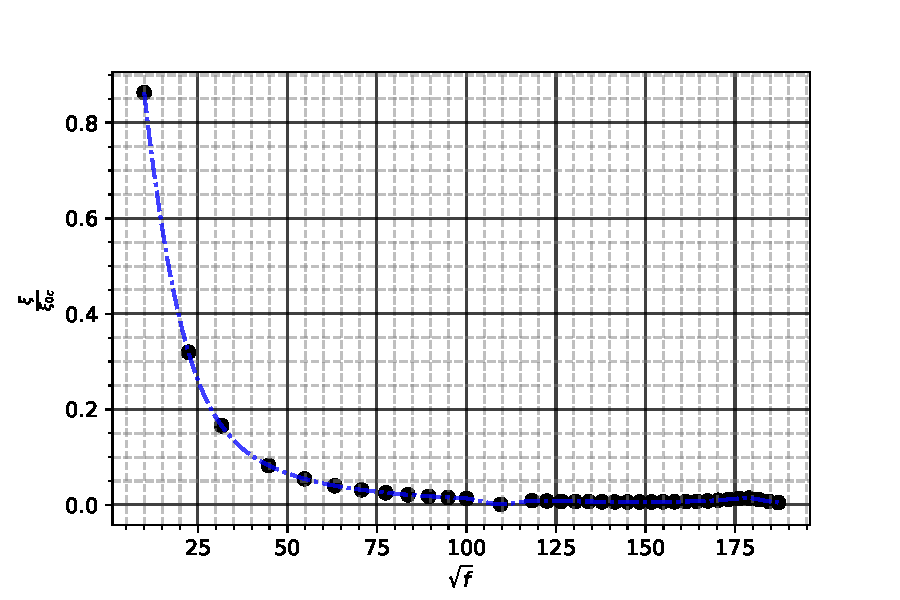
\includegraphics[width = \textwidth]{xi_xi0(sqrt).pdf}
        \caption{График зависимости $\frac{|H_{1}|}{|H_{0}|}$ от $\sqrt{f}$}
        \label{xi_xi0(sqrt)}
    \end{figure}

    Расчитаем аналогичную теоретическую зависимость по формуле

    \begin{equation}
        H_{1} = \frac{2 H_0}{a k \sh{k h} + 2 \ch{k h}}
    \end{equation}

    где
    \begin{equation}
        \delta = \sqrt{\frac{1}{\pi \mu_0 \mu \sigma f}} = \sqrt{\frac{1}{\pi \mu_0 \sigma f}}
    \end{equation}
    глубина проникновения, а
    \begin{equation}
       k = \frac{1 + i}{\delta} 
    \end{equation}

    Стоит воспользоваться приближением при низких и высоких частотах. 
    При низких частотах выражение приближается формулой 
    \begin{equation}
        \frac{|H_1|}{|H_0|} = \frac{1}{\sqrt{1 + \frac{1}{4} (2 \pi a h \sigma \mu_0 f)^2}}
    \end{equation}

    При высоких частотах 
    \begin{equation}
        \frac{|H_1|}{|H_0|} = \frac{2 \sqrt{2} \delta}{a} e^{-\frac{h}{\delta}}
    \end{equation}

    Полученная таким образом теоретическая зависимость достаточно хорошо ложится на экспериментальные данные.

    \begin{figure}
        \centering
        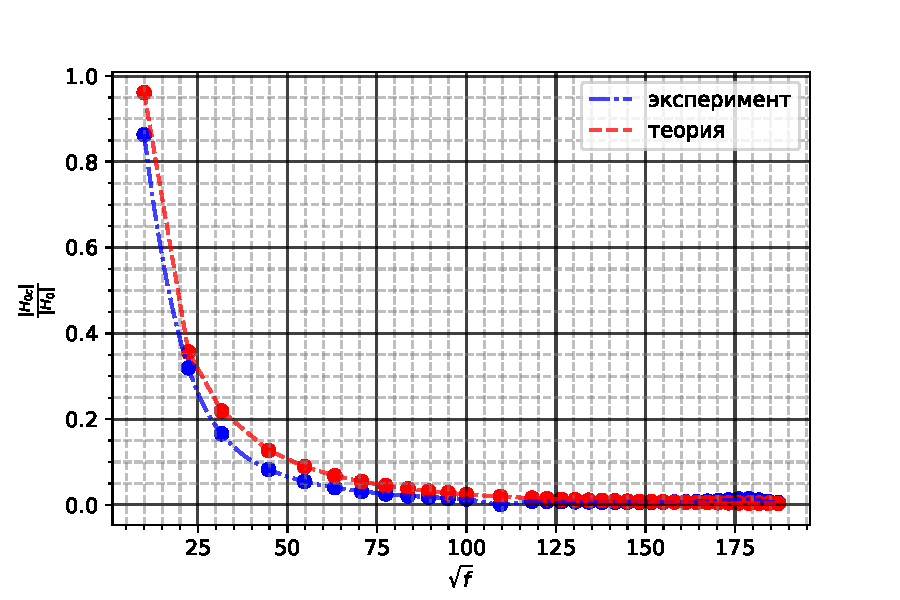
\includegraphics[width = \textwidth]{exp_th(sqrt).pdf}
        \caption{Сравнение экспериментальной зависимости с теоретической}
        \label{exp_th(sqrt)}
    \end{figure}

    Воспользовавшись найденным значением $\sigma$, вычислим глубину проникновения $\delta$ при частотах 50 Гц и $10^5$ Гц.

    \begin{center}
        На частоте 50 Гц глубина проникновения $\delta = (9.89 ~ \pm ~ 0.68)$ мм \\
        На частоте $10^5$ Гц глубина проникновения $\delta = (22.0 ~ \pm ~ 1.5) \cdot 10^{-2}$ мм
    \end{center}

	\section*{Вывод}

	В данной работе было исследовано явление скин-эффекта. Была найдена глубина проникновения магнитного поля в полый медный цилиндр при разных частотах генератора. Мы убедились, что данная зависимость $\delta (f)$ является обратно корневой: $\delta (f) \propto \frac{1}{\sqrt{f}}$. Была найдена удельная проводимость меди $\sigma = (5.18 \pm 0.71)\cdot 10^7$ См/м, что является $\thicksim 80\%$ от табличного значения, то есть меньше него, как и было заявлено. Зависимость фазы $\Delta \psi (\sqrt{f})$ также неплохо ложится на предсказанную прямую, но имеет небольшое отклонение при $f \thicksim 10$ кГц и достаточно сильное отклонение в большую сторону при частотах $f \thicksim 30-31$ кГц -- это резонансы. Экспериментальное подтверждение получила и зависимость отношения амплитуд поля $\frac{|H_1|}{|H_0|}(\sqrt{f})$ от корня частоты, хоть она и является достаточно сложной. Несмотря на точные электронные приборы, систематические погрешности никуда не делись -- согласно паспортным данным приборов, они составляют $0.1\%$ и $0.2\%$ для вольтметра и амперметра соответственно. Вдобавок случайные погрешности также вносят свой вклад в общие, а потому последние составляют $\thicksim 10\%$ от значения. Несмотря на все это, теория скин-эффекта хорошо предсказывает качественное поведение поля в цилиндре, хоть и имеет количественные неточности.
    
\end{document}